\documentclass[a4paper,12pt]{article}
\usepackage[utf8]{inputenc}
\usepackage{enumitem}
\usepackage{amsmath}
\usepackage{graphicx}
\usepackage{listings}
\usepackage{hyperref}
\usepackage{fancyhdr}
\usepackage{titlesec}
\usepackage{times}
\usepackage{courier}
\usepackage{float}
\usepackage[top=1in, bottom=1in, left=0.5in, right=0.5in]{geometry}
\renewcommand{\baselinestretch}{1}

\pagestyle{fancy}
\fancyhf{}
\fancyfoot[C]{\thepage}

\titleformat{\section}{\normalfont\Large\bfseries}{\thesection}{1em}{}
\titleformat{\subsection}{\normalfont\large\bfseries}{\thesubsection}{1em}{}
\titleformat{\subsubsection}{\normalfont\normalsize\bfseries}{\thesubsubsection}{1em}{}

\lstset{
  basicstyle=\ttfamily,
  numbers=left,
  numberstyle=\tiny,
  stepnumber=1,
  numbersep=5pt,
  showspaces=false,
  showstringspaces=false,
  showtabs=false,
  frame=single,
  tabsize=2,
  breaklines=true,
  breakatwhitespace=false,
  captionpos=b
}

\begin{document}

\begin{titlepage}
    \centering
    {\huge\bfseries Crypto Trading Platform \par}
    \vspace{0.5cm}
    {\Large Trading 212 Project \par}
    \vspace{1.5cm}
    {\large Akaga Radoslavova Pavlova \par}
    \vfill
    {\large \today \par}
\end{titlepage}

\tableofcontents
\newpage

\section{Overview}
\subsection{Project Description}
This project simulates a cryptocurrency trading platform via a web application. It allows users to view real-time prices of the top 20 cryptocurrencies, manage a virtual balance, execute trades, and track their transaction history.

\subsection{Functionality}
\begin{itemize}[label=-, itemsep=0.2em]
    \item Dynamically update top 20 cryptocurrency prices in real-time via Kraken WebSocket API.
    \item Present crypto name, symbol, and price in a table or list format.
    \item Initialize a virtual account balance.
    \item Buy/sell crypto with balance checks and updates.
    \item Track and log all transactions per user.
    \item Reset user portfolio to the initial state.
    \item Display proper error handling and feedback messages.
\end{itemize}

\subsection{Technical Stack}
\begin{itemize}[label=-, itemsep=0.2em]
    \item Frontend: React (HTML, CSS, JS).
    \item Backend: Java with Spring Boot.
    \item WebSocket Integration: Kraken API (V2).
    \item Database: MySQL (manual SQL schema).
\end{itemize}

\subsection{Documentation Structure}
This documentation covers the architecture, backend implementation (DAO classes, services), integration with external APIs, database structure, and testing procedures.

\section{Domain Model}
\subsection{Key Concepts}
\begin{itemize}
    \item \textbf{User} – Has a unique account with balance and crypto holdings.
    \item \textbf{CryptoCoin} – Represents a tradable cryptocurrency.
    \item \textbf{Transaction} – A record of a buy/sell/withdraw/deposit operation performed by a user.
    \item \textbf{WebSocket Listener} – Subscribes to Kraken's real-time price updates.
    \item \textbf{Portfolio} – Tracks account data (balance/coins/gains/transaction history) for the user.
\end{itemize}

\subsection{Challenges}
\begin{itemize}
    \item Backend-frontend-DB separation : logic vs presentation vs data maintainability.
    \item Real-time communication using WebSocket API.
    \item Transaction validation (balance, holdings).
    \item SQL schema creation and consistency without ORM.
\end{itemize}

\subsection{Approach}
\begin{itemize}
    \item Backend handles all business logic (Spring Boot).
    \item Frontend request backend on demand - on user interaction and dynamically update prices via WebSocket listener (later the latter ligic should be moved to the backend) (React).
    \item MySQL used for persistent state: users, coins, transactions.
    \item DAO pattern for low-level database access.
\end{itemize}

\section{Architecture}
\subsection{Overall Design}
The system is built using a client-server architecture. The frontend is responsible for rendering data and user interactions. The backend performs data processing, state management, and interacts with the database (later on it would manage the external API).

\subsection{Database Schema}
Tables:
\begin{itemize}
    \item \texttt{Users (Id, userName, dateOfRegistration, Balance)}
    \item \texttt{CryptoCoins (Symbol, Price)}
    \item \texttt{Transactions (Id, Name, Type, DateOfTransaction, CryptoSymbol, CryptoType, Amount)}
    \item \texttt{HasCoins (UserId, CoinId, Amount)}
    \item \texttt{HasDoneTransactions (UserId, TransactionId)}
\end{itemize}

\section{Implementation}
\subsection{Backend - DAO Classes}
\subsubsection{UserDAO}
Handles SQL operations on the \texttt{Users} table: create, update balance, fetch user details.

\begin{lstlisting}[language=Java]
public class UserDAO {
    public List<Transaction> getTransactionsByUserId(int userId)
    public void updateBalanceById(int userId, double newBalance);
    public Double getTotalGains(User user);
    public List<Holding> getAllHoldingsByUserId(int userId);
    ...
}
\end{lstlisting}

\subsubsection{TransactionDAO}
Manages user transactions and joins with the Transactions table.

\begin{lstlisting}[language=Java]
public class TransactionDAO {
    public void deleteAllTransactionsByUser(int userId);
    public List<Transaction> getTransactionsByUserId(int userId);
    public void save(Transaction transaction);
    ...
}
\end{lstlisting}

\subsubsection{CryptoCoinDAO}
Handles operations for CryptoCoins table.

\begin{lstlisting}[language=Java]
public class CryptoCoinDAO {
    public List<CryptoCoin> getAllCoins();
    public CryptoCoin getCoinBySymbol(String symbol);
    ...
}
\end{lstlisting}
...

\subsection{Backend Services}
% \subsubsection{WebSocketService}
% Establishes connection with Kraken API and listens for price updates.

% \begin{lstlisting}[language=Java]
% @Scheduled(fixedDelay = 10000)
% public void subscribeToKrakenWebSocket() {
%     // Build subscription message and connect to Kraken
% }
% \end{lstlisting}

\subsubsection{TradingService}
Contains business logic for buy/sell operations.

\begin{lstlisting}[language=Java]
public class TradingService {
    public String buy(int userId, TradeRequest request);
    public String sell(int userId, TradeRequest request);
    ...
}
\end{lstlisting}

\subsection{Frontend Integration}
React sends requests to Spring Boot backend via REST API.
\begin{itemize}
    
    \item \texttt{GET \$\{BASE\}/trade/\$\{userId\}/withdraw}
    \item \texttt{POST \$\{BASE\}/trade/\$\{userId\}/deposit}
    \item \texttt{POST \$\{BASE\}/trade/\$\{userId\}/buy}
    \item \texttt{GET \$\{BASE\}/trade/\$\{userId\}/sell}
    \item \texttt{GET \$\{BASE\}/user/\$\{userId\}/transactions}
    \item \texttt{GET \$\{BASE\}/user/\$\{userId\}/gains}
    \item \texttt{GET \$\{BASE\}/user/\$\{userId\}/holdings}
    \item \texttt{GET \$\{BASE\}/user/\$\{userId\}/reset}
    \item \texttt{should be integrated: {GET \$\{BASE\}/market/prices}}
\end{itemize}

\section{Testing}
\subsection{Frontend Integration Testing}
Frontend React application was tested manually via the browser. The following screenshots show different stages of user interaction:

\begin{figure}[H]
    \centering
    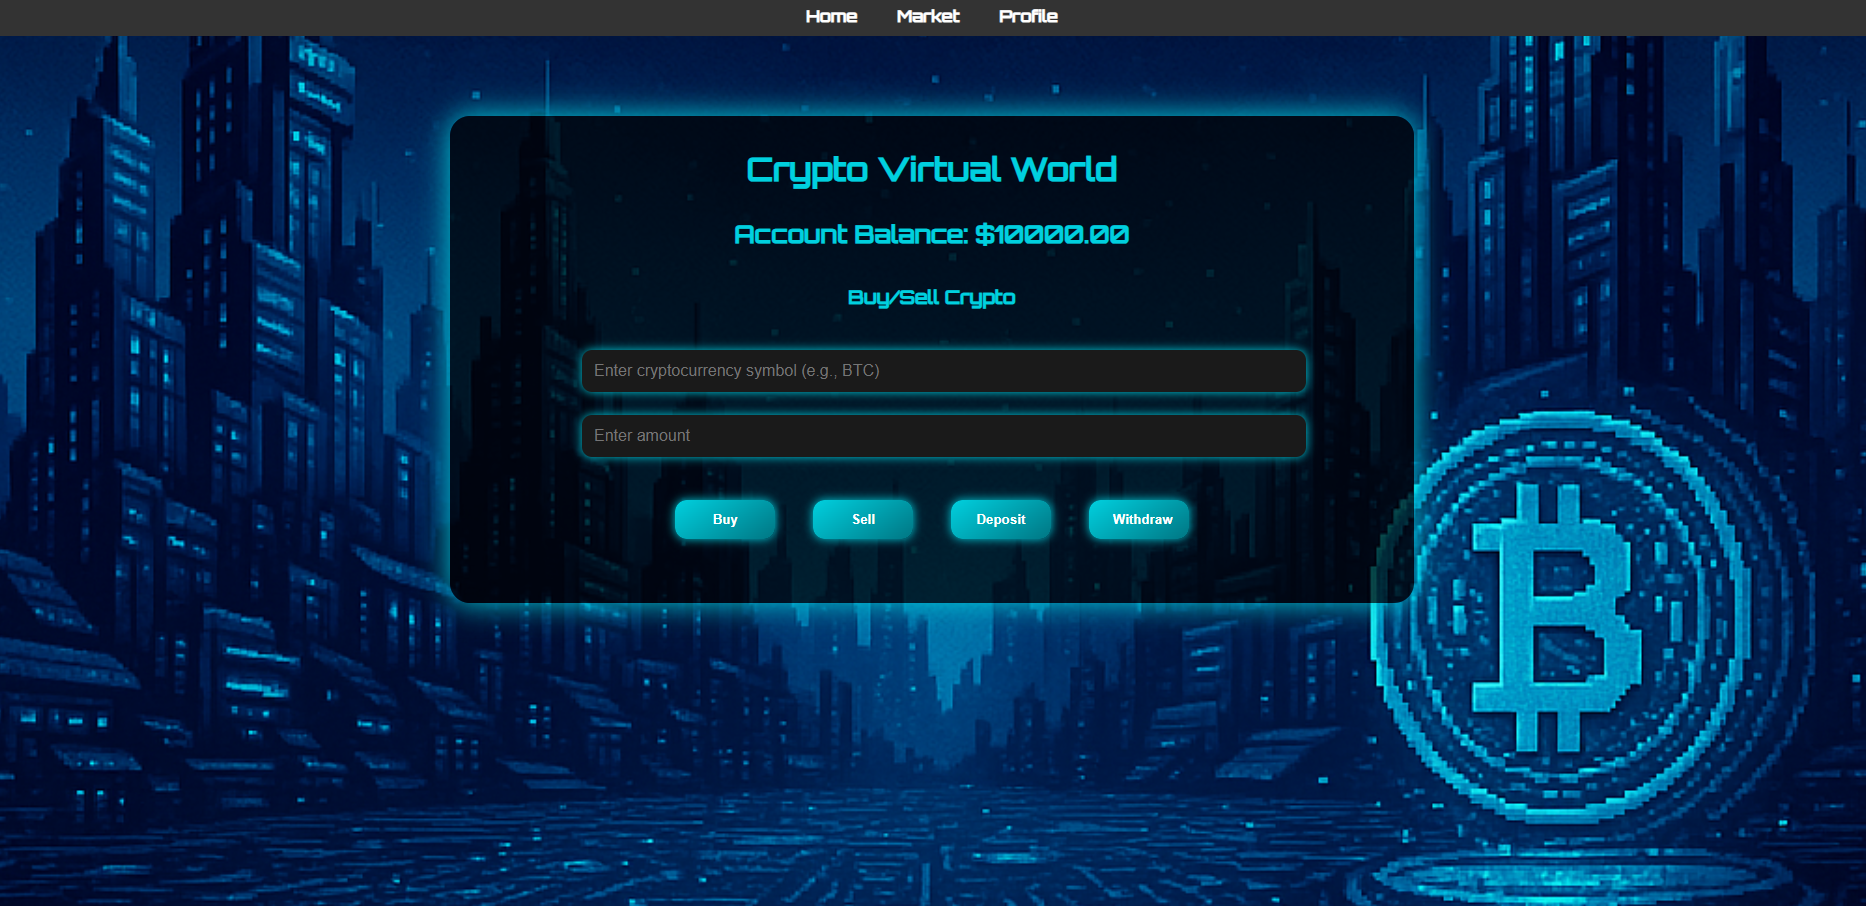
\includegraphics[width=1.0\textwidth]{homePage.png}
    \caption{Home Page – General view}
\end{figure}

\begin{figure}[H]
    \centering
    \includegraphics[width=1.0\textwidth]{buy.png}
    \caption{Successful buy view – User bought 10 ADA coins}
\end{figure}

\begin{figure}[H]
    \centering
    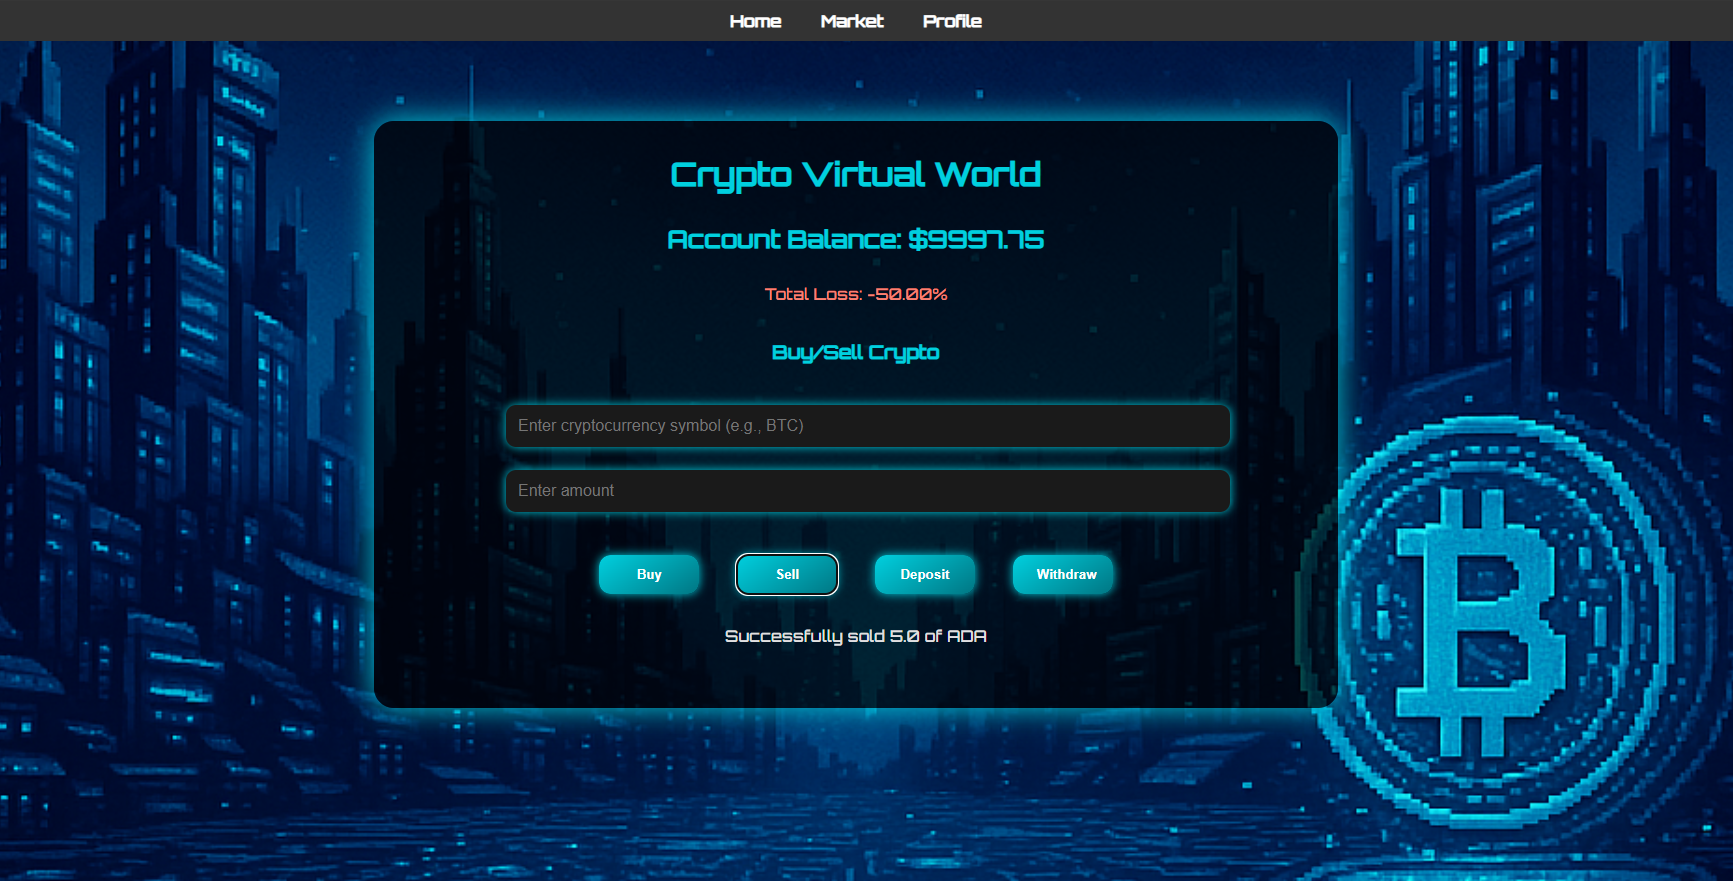
\includegraphics[width=1.0\textwidth]{sell.png}
    \caption{Successful sell view – User sold 5 ADA coins}
\end{figure}

\begin{figure}[H]
    \centering
    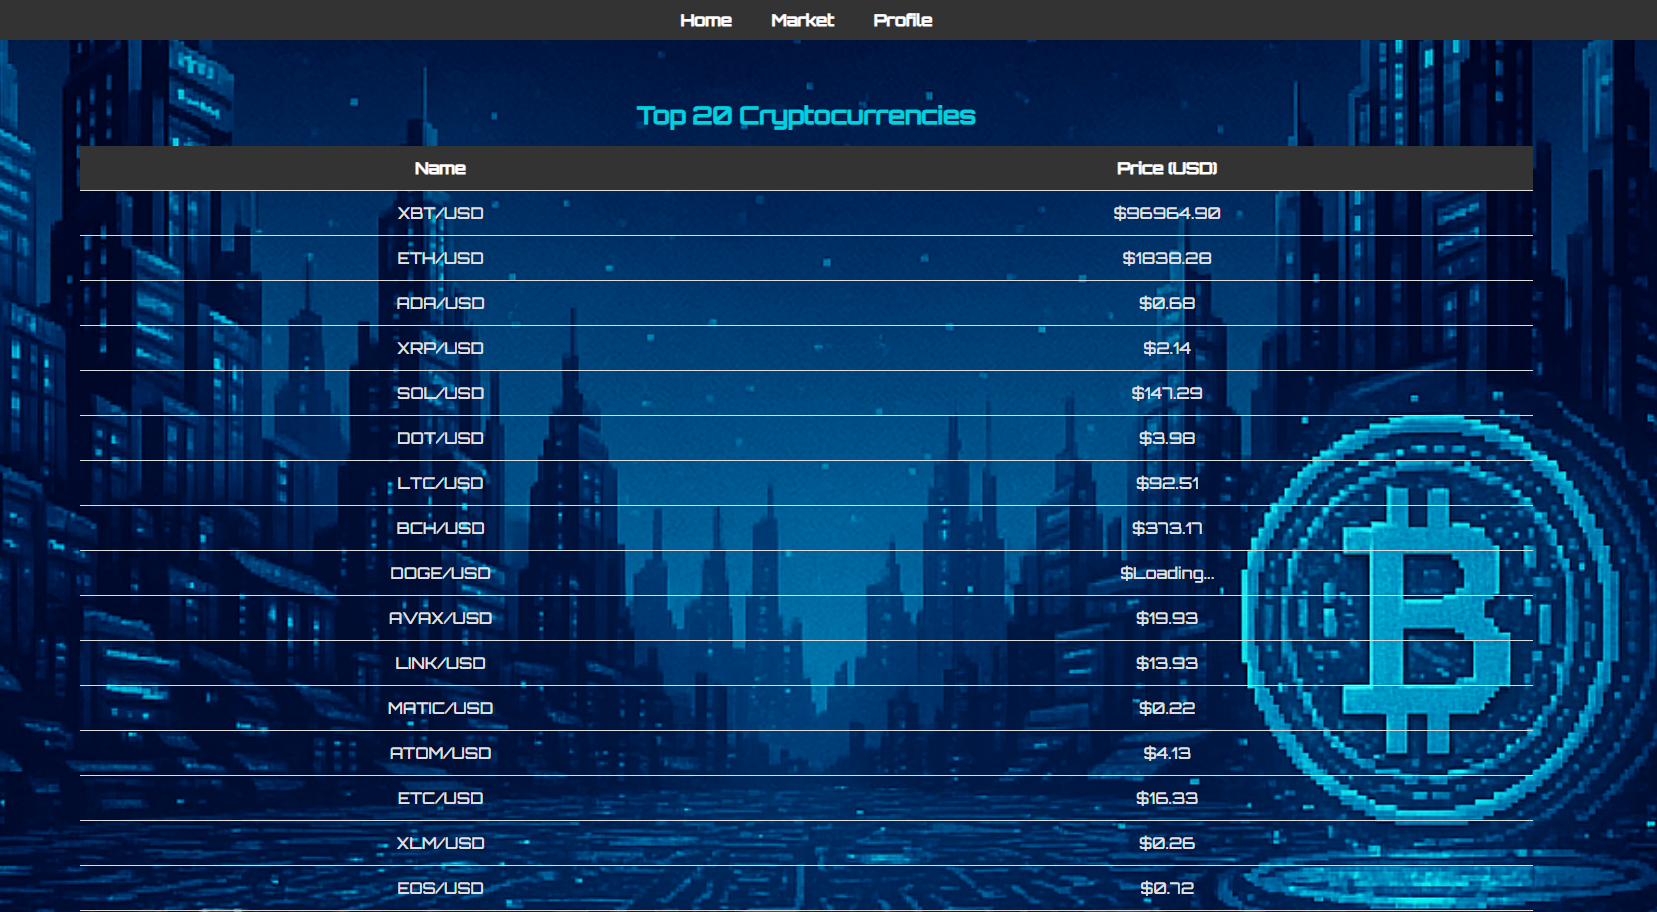
\includegraphics[width=1.0\textwidth]{market.png}
    \caption{Market – Top 20 crypto coins with their values}
\end{figure}

\begin{figure}[H]
    \centering
    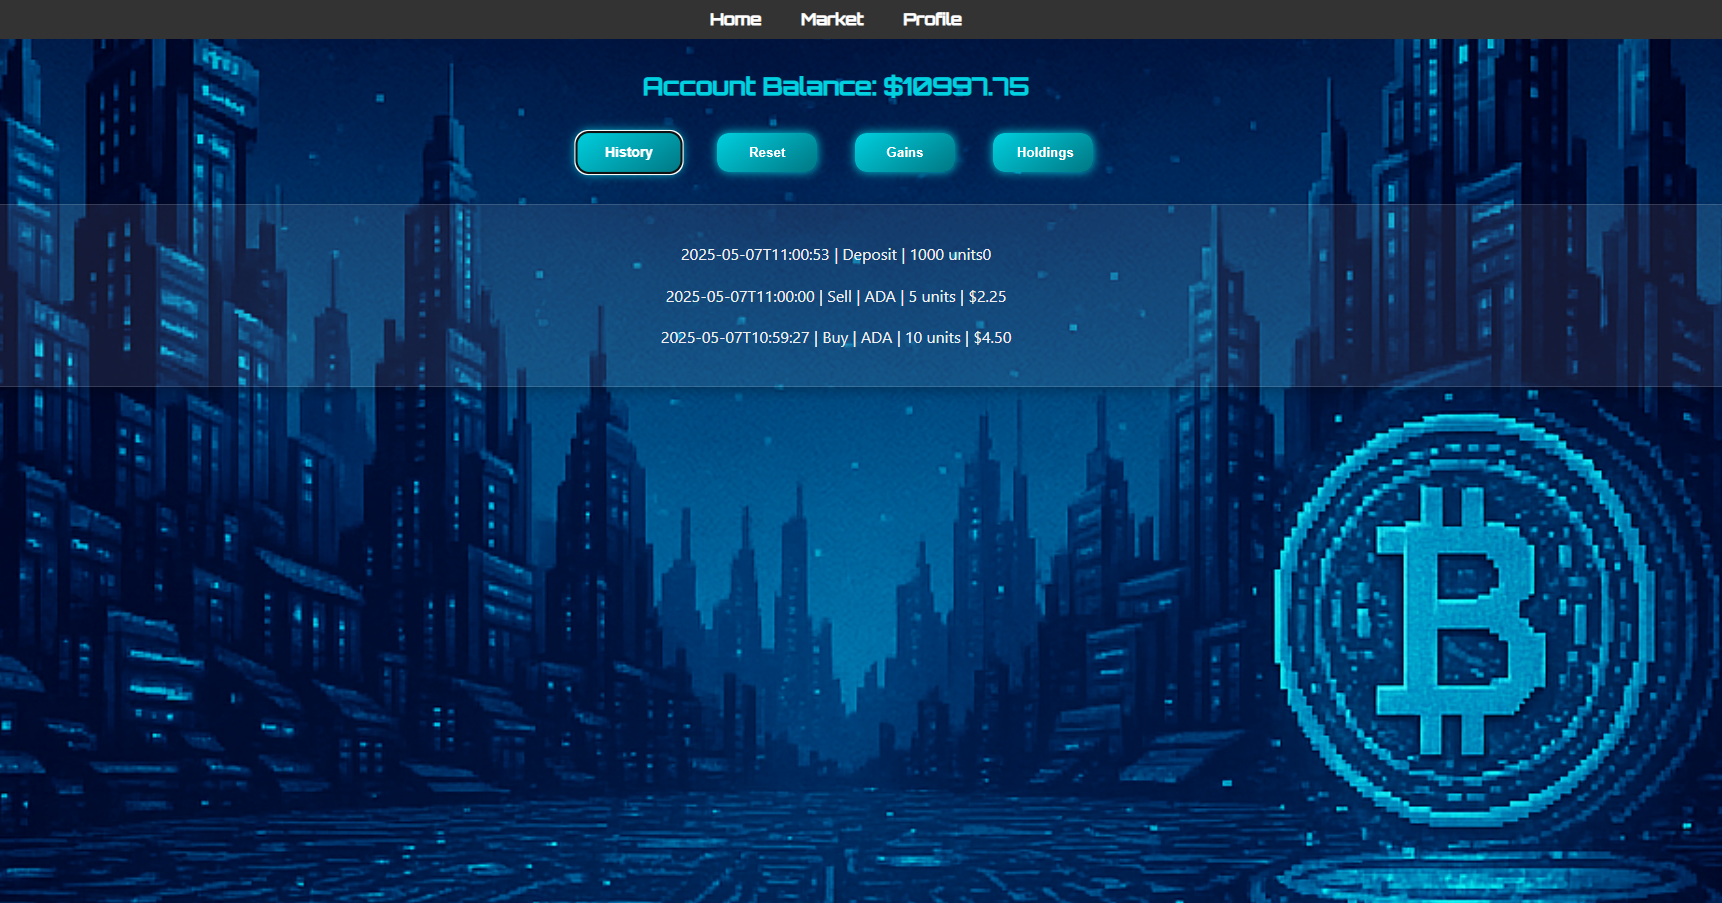
\includegraphics[width=1.0\textwidth]{transactions.png}
    \caption{Transaction History – Past trades are shown with timestamps and values}
\end{figure}

\section{Dependencies}

This project relies on the following frameworks, APIs, and tools:

\subsection{Backend Dependencies (Java Spring Boot)}
\begin{itemize}[label=-, itemsep=0.2em]
    \item \textbf{Spring Boot} – Core framework for building REST APIs.
    \item \textbf{Spring Web} – For building HTTP endpoints.
    \item \textbf{Spring JDBC} – Used for direct interaction with MySQL without ORM.
    \item \textbf{MySQL Tools} – Client for MySQL database access.
    \item \textbf{Jackson} – For JSON serialization/deserialization.
\end{itemize}

\subsection{Frontend Dependencies (React)}
\begin{itemize}[label=-, itemsep=0.2em]
    \item \textbf{React} – JavaScript library for building user interfaces.
    \item \textbf{Fetch API} – For HTTP communication with backend.
\end{itemize}

\subsection{External Services}
\begin{itemize}[label=-, itemsep=0.2em]
    \item \textbf{Kraken WebSocket API (v2)} – Real-time crypto price streaming.
    \item \textbf{MySQL Database (v8+)} – Stores users, crypto coins, transactions, and portfolios.
\end{itemize}


\section{Conclusion}
\subsection{Summary}
The system successfully meets basic requirements simulating a cryptocurrency trading platform with real-time updates, backend-driven logic, and persistent user and transaction data.

\subsection{Future Improvements}
\begin{itemize}
    \item Add user authentication and session management.
    \item Expand to more cryptocurrencies and exchanges.
    \item Add analytics features: gain/loss ratio, price history.
    \item Add test cases
\end{itemize}

\end{document}
